\documentclass[tikz,border=8pt]{standalone}
% Shared TikZ style for synorg platform diagrams. Each diagram \input's this
% inside a standalone document. Palette tracks the Material "teal" site theme so
% figures read as one system in light mode (SVGs are theme-neutral otherwise).
\usetikzlibrary{arrows.meta,positioning,shapes.geometric,fit,backgrounds,calc,decorations.pathreplacing}

\definecolor{synteal}{HTML}{00897B}   % primary
\definecolor{synfill}{HTML}{E0F2F1}   % light fill
\definecolor{synamber}{HTML}{B26A00}  % warning / lend
\definecolor{synred}{HTML}{B00020}    % deny / danger
\definecolor{syngrey}{HTML}{5F6368}   % muted

\tikzset{
  >=Stealth,
  font=\sffamily\small,
  box/.style={draw=synteal,line width=0.6pt,rounded corners=2pt,fill=synfill,
              inner sep=5pt,align=center},
  plane/.style={draw=synteal,line width=0.8pt,rounded corners=3pt,fill=synfill,
                inner sep=8pt,align=center},
  state/.style={draw=synteal,line width=0.7pt,circle,fill=synfill,inner sep=3pt,
                minimum size=11mm,align=center,font=\sffamily\footnotesize},
  decision/.style={draw=synteal,line width=0.7pt,diamond,aspect=2,fill=synfill,
                   inner sep=1pt,align=center,font=\sffamily\footnotesize},
  deny/.style={draw=synred,fill=synred!8,text=synred},
  warn/.style={draw=synamber,fill=synamber!10},
  flow/.style={->,line width=0.6pt,draw=syngrey},
  flowlbl/.style={font=\sffamily\footnotesize,text=syngrey,inner sep=2pt},
  note/.style={font=\sffamily\footnotesize\itshape,text=syngrey},
}

\begin{document}
% The lend/reclaim lifecycle a GPU node moves through — the state machine the
% lending controller owns (operations.md, architecture.md).
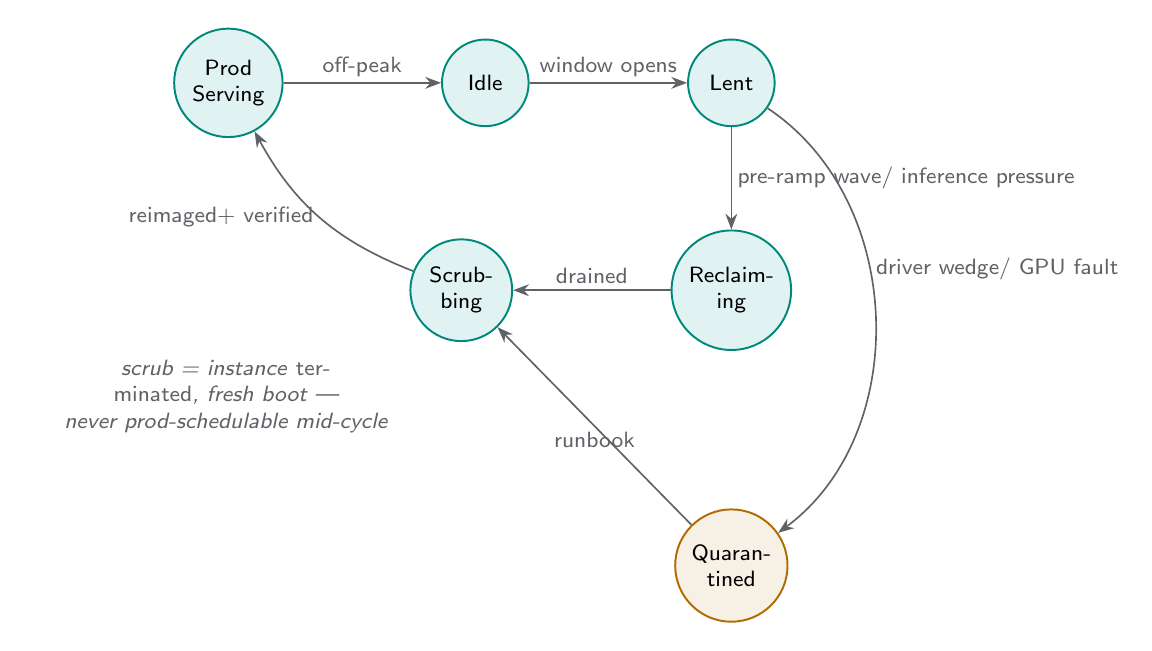
\begin{tikzpicture}[node distance=13mm and 20mm]
  \node[state] (prod) {Prod\\Serving};
  \node[state,right=of prod] (idle) {Idle};
  \node[state,right=of idle] (lent) {Lent};
  \node[state,below=of lent] (recl) {Reclaim-\\ing};
  \node[state,left=of recl] (scrub) {Scrub-\\bing};
  % Quarantined is the fault branch off Lent; drop it a full row below
  % Reclaiming so it never lands on Scrubbing (it did when placed under Idle).
  \node[state,warn,below=20mm of recl] (quar) {Quaran-\\tined};

  \draw[flow] (prod) -- node[flowlbl,above]{off-peak} (idle);
  \draw[flow] (idle) -- node[flowlbl,above]{window opens} (lent);
  \draw[flow] (lent) -- node[flowlbl,right]{pre-ramp wave\\/ inference pressure} (recl);
  \draw[flow] (recl) -- node[flowlbl,above]{drained} (scrub);
  \draw[flow] (scrub) to[bend left=20] node[flowlbl,left]{reimaged\\+ verified} (prod);
  \draw[flow] (lent) to[bend left=55] node[flowlbl,right,pos=0.4]{driver wedge\\/ GPU fault} (quar);
  \draw[flow] (quar) -- node[flowlbl,below,align=center]{runbook} (scrub);

  % Note sits under Scrubbing (upper-left of the lower area); Quarantined is
  % under Reclaiming (right) — they clear each other.
  \node[note,below left=3mm and 0mm of scrub,text width=48mm,align=center]
    {scrub = instance \emph{terminated}, fresh boot —\\ never prod-schedulable mid-cycle};
\end{tikzpicture}
\end{document}
